\chapter{Reprodukcja}\label{metody_reprodukcji}

Jednym z~etapów algorytmu ewolucyjnego jest~reprodukcja polegająca na~wyborze osobników, które~przedostaną się~do~grupy rozrodczej tworzącej potomstwo. W~klasycznym algorytmie ewolucji różnicowej wybór wektorów bazowych oraz~wektorów składających się~na~wektor różnicowy jest~dokonywany losowo \cite{diff2}. Nie~mniej jednak w~niniejszej pracy w~celach doświadczalnych zostaną porównane i~zestawione ze~sobą dodatkowo metody doboru grupy rodzicielskiej zgodnie z~dostępnymi metodami selekcji stosowanymi w~algorytmach ewolucyjnych.\\

Znanych jest~kilka metod selekcji, na~podstawie których dokonuje się~wyboru osobników z~różnym prawdopodobieństwem. Metody te~w~większości zostały opracowane w~taki sposób, by~dawały większe szanse przetrwania osobnikom lepiej do~tego przystosowanym, a~więc osobnikom o~większym współczynniku funkcji przystosowania. Metody selekcji zostały zaimplementowane w~dwojaki sposób. Pierwszym z~nich jest~możliwość pojawienia się~danego osobnika w~grupie rodzicielskiej więcej niż jeden raz. Druga technika nakazuje różnorodność osobników w~obrębie danej instancji grupy rozrodczej.\\

\begin{equation}
i_{1} \ne i_{2} \ne i_{3} \ne ... \ne i_{n}
\end{equation}
Gdzie:\\
$i_{n}$ - n-ty osobnik\\

Poniżej przestawiono idee metod selekcji podlegających rozważaniom w~ramach tej pracy. Implementacje metod powstały w~oparciu o~\cite{maszynowe_sel}, \cite{gracjan}. Listingi poszczególnych metod reprodukcji można znaleźć w~dodatku \ref{reporeprodukcji}.

%---------------------------------------------------------------------------

\section{Klasyczna reprodukcja : Losowy wybór}\label{sec:strukturaDokumentu}

Z~populacji wybierany jest~osobnik przechodzący do~grupy rozrodczej w~oparciu o~wylosowaną liczbę odpowiadającą indeksowi konkretnego osobnika. Metoda ta jest~niezależna od~wartości funkcji przystosowania, a~więc daje równe szanse każdemu z~osobników. Prawdopodobieństwo wylosowania danego osobnika, z~populacji składającej się~z~$n$ osobników, jest~równe:
\vspace{0,4cm}
\begin{equation}
P = \frac{1}{n}
\end{equation}

%---------------------------------------------------------------------------

\section{Modyfikacje reprodukcji}\label{sec:kompilacja}
\subsection{Metoda rankingowa}\label{sec:kompilacja}


W~metodzie selekcji rankingowej dla~osobników składających się~na~populacje rodziców obliczana jest~wartość funkcji celu, na~której to~podstawie tworzony jest~ranking. Osobniki z~najmniejszą wartością wyniku uzyskują najwyższe miejsca w~rankingu \cite{selekcje}. Miejsce w~rankingu jest~argumentem funkcji, na~podstawie której~obliczane jest~prawdopodobieństwo wyboru danego osobnika jako rodzica. Rodzic zostanie poddany kolejnym operacjom (mutacja, krzyżowanie).\\
Funkcja stosowana, na~której to~podstawie tworzony jest~ranking, może być~funkcją liniową. Wówczas osobniki zajmujące w~rankingu będącym $n$ elementowym wektorem konkretne miejsce określone rangą, gdzie $n$  to~ilość osobników w~populacji otrzymują prawdopodobieństwo przejścia do~grupy rodzicielskiej określone zależnością \ref{wzorranking}:
\begin{equation}
P = \frac{ranga}{\sum_{j=1}^{n}j}
\label{wzorranking}
\end{equation}

\begin{table}[h!]
\begin{center}
\caption{Wartości parametrów na kolejnych osobników w metodzie rankingowej.}
\begin{tabular}{|c|c|c|c|}
\hline
\textbf{Osobnik}  & \textbf{Funkcja celu} & \textbf{Ranga} & \textbf{Prawdopodobieństwo}\\
\hline
Osobnik 1 & 373 & 1 & 6,(6) \% \\
\hline
Osobnik 2 &254 & 2  & 13,(3)  \% \\
\hline
Osobnik 3 & 202 & 3 & 20  \% \\
\hline
Osobnik 4 & 136 & 4 & 26,(6)  \% \\
\hline
Osobnik 5 & 10 & 5 & 33,(3)  \% \\
\hline
\end{tabular}
\end{center}
\end{table}

\vspace{0,4cm}

\begin{figure}[h]
		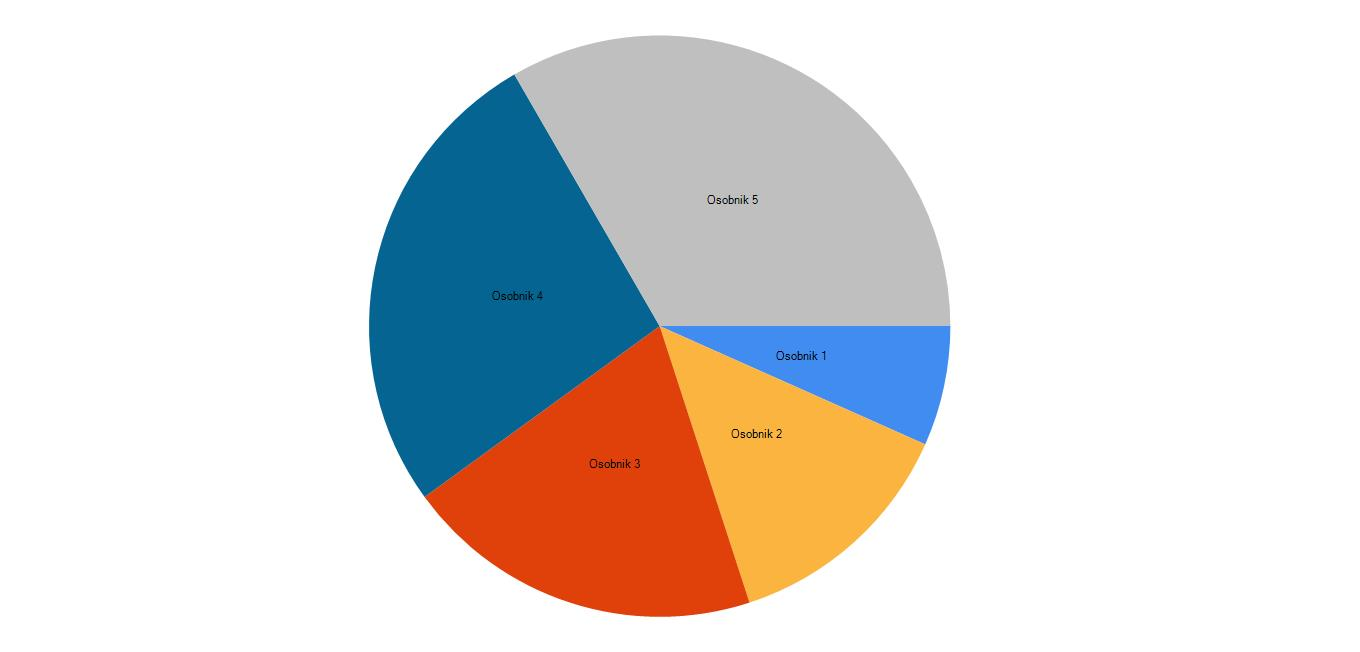
\includegraphics[scale=0.45]{../../../../Screeny/metoda_rankingowa.jpg}
		\caption{Rozkład prawdopodobieństwa w~metodzie rankingowej.}
		\label{rankingR}			
\end{figure}
\par
Na~podstawie \ref{rankingR} zauważalny staje się~fakt, iż~rozkład prawdopodobieństwa nie~jest~bezpośrednio zależny od~wartości funkcji celu. W~metodzie tej zwiększone są~więc szanse przejścia do~grupy rodzicielskiej osobników z~małą wartością funkcji dopasowania, które~to miałyby małe szanse przejścia dalej w~metodzie selekcji zależnej od~wartości funkcji celu. Metoda może wydawać się~niekorzystna z~punktu widzenia osobników z~dużą wartością funkcji dopasowania, jako że~mogą otrzymać one niewiele większe prawdopodobieństwo przejścia do~grupy rodzicielskiej od~osobników znajdujących się~rangę niżej, pomimo iż~ich wartości funkcji celu mogą różnić się~znacząco.
%---------------------------------------------------------------------------

\subsection{Metoda ruletki}\label{sec:narzedzia}


W~metodzie ruletki każdemu chromosomowi zostaje przypisany wycinek koła \cite{selekcje}. Im silniejszy osobnik, tym większy wycinek koła dostaje, gdyż zależność wartości funkcji przystosowania i~prawdopodobieństwo wylosowania osobnika jest~wprost proporcjonalna. Każdy osobnik tworzący populacje poddawany jest~ocenie funkcji celu. Maksymalna wartość funkcji przystosowania oznacza najmniejszą wartość funkcji celu. Uzyskana wartość funkcji przystosowania w~stosunku do~sum wartości tej funkcji wszystkich osobników populacji wyznacza prawdopodobieństwo wylosowania danego osobnika na~rodzica. Prawdopodobieństwo wylosowania danego osobnika dane jest~następującą zależnością:
\begin{equation}
P_i = \frac{f(i)}{\sum_{j=1}^{n}f(j)}
\end{equation}
Gdzie f(x) - funkcja przystosowania\\
\par
Funkcją przystosowania w~rozważanym poniżej przypadku jest~funkcja przyporządkowującą największej wartości funkcji celu wartość najmniejszą, a~wartości najmniejszej wartość największą.

\begin{table}[h!]
\begin{center}
\caption{Wartości parametrów na kolejnych osobników w metodzie ruletki.}
\begin{tabular}{|c|c|c|c|}
\hline
\textbf{Osobnik}  & \textbf{Funkcja celu} & \textbf{Funkcja dopasowania} & \textbf{Prawdopodobieństwo}\\
\hline
Osobnik 1 & 373 & 10 & 1,02  \% \\
\hline
Osobnik 2 &254 & 136  & 13,95  \% \\
\hline
Osobnik 3 & 202 & 202 & 20,72  \% \\
\hline
Osobnik 4 & 136 & 254 & 26,05  \% \\
\hline
Osobnik 5 & 10 & 373 & 38,25  \% \\
\hline
\end{tabular}
\end{center}
\end{table}

\vspace{0,4cm}

\begin{figure}[h]
		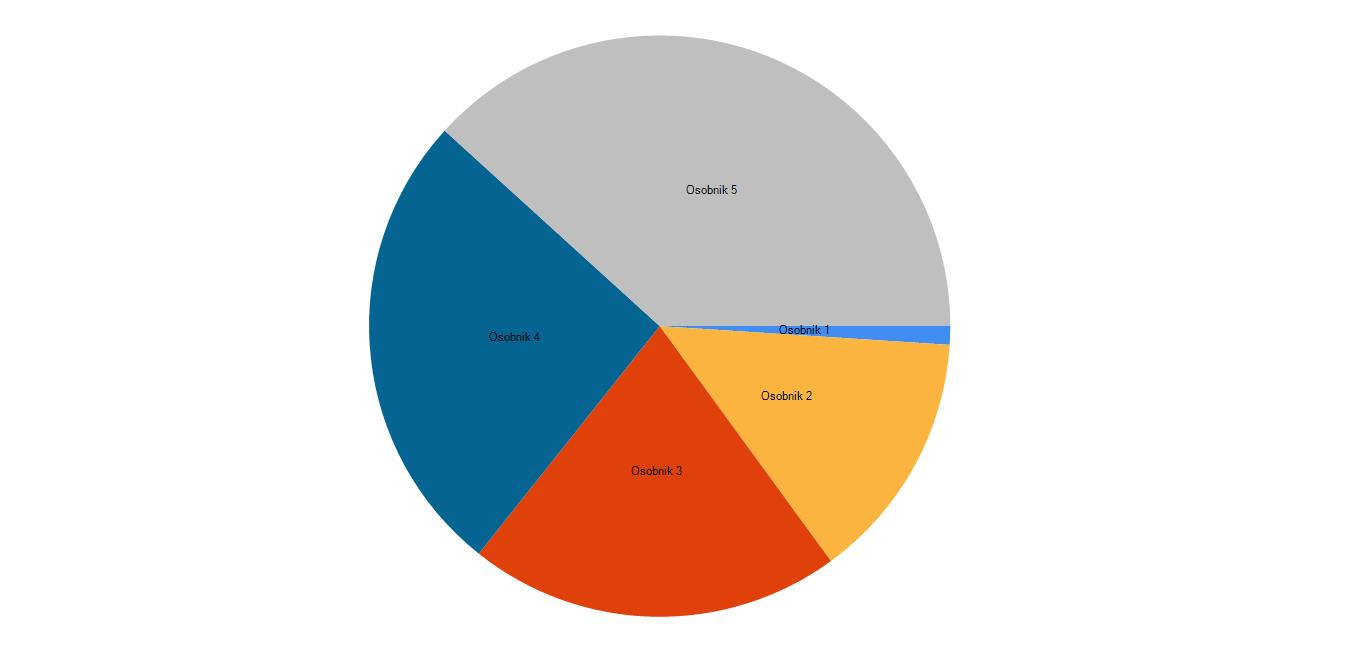
\includegraphics[scale=0.45]{../../../../Screeny/metoda_ruletki.jpg}
		\caption{Rozkład prawdopodobieństwa w~metodzie ruletki.}
		\label{ruletka}			
\end{figure}
\par
W~metodzie ruletki wkład każdego osobnika w~rozkład prawdopodobieństwa jest~wprost proporcjonalny do~wartości jego funkcji dopasowania. Wady tej metody stają się~widoczne, w~sytuacji, gdy dany osobnik zajmuje większość powierzchni koła, gdyż osobniki o~małej wartości funkcji dopasowania są~przedwcześnie eliminowane, a~więc nie~mają wielkiej szansy, by~zostać wylosowane. Prowadzi to~do~braku różnorodności w~kolejnych grupach rozrodczych, co utrudnia dojście do~lepszego wyniku. Z~problemem tym dobrze sobie radzi wspomniana wyżej metoda rankingowa, gdzie eliminowana jest~możliwość dużej przewagi jednego z~nich nad~resztą.\\
%---------------------------------------------------------------------------

\subsection{Metoda turniejowa}\label{sec:narzedzia}


Metoda selekcji turniejowej polega na~rozgrywaniu turnieju pomiędzy osobnikami tworzącymi populacje. W~wyniku jednorazowej rozgrywki wygrywa osobnik o~większej wartości funkcji przystosowania, przechodząc tym samym do~kolejnej rundy. W~każdym turnieju zwycięża jeden osobnik, którego~to genotyp jest~wykorzystywany przy kolejnych operacjach genetycznych. Populacja dzielona jest~na~podgrupy złożone z~dwóch osobników, w~których to~dokonywane są~rozgrywki. W~przypadku nieparzystego rozmiaru populacji osobnik ostatni przechodzi do~kolejnej rundy bezkonkurencyjnie. \\
\par
Metoda turniejowa nie~wymaga znajomości optymalizowanej funkcji, konieczny jest~jedynie informacja o~relacji zachodzącej pomiędzy dwoma kolejnymi osobnikami. 
%---------------------------------------------------------------------------

\subsection{Metoda elitarna}\label{sec:przygotowanieDokumentu}

W~metodzie tej nacisk położony jest~na~to, aby~do~grupy rozrodczej przedostały się~z~prawdopodobieństwem równym p=100\% osobniki najlepiej przystosowane. W~poprzednich metodach (ruletki, turniejowa, rankingowa) prawdopodobieństwo przejścia do~grupy rozrodczej dla~osobników z~większym wskaźnikiem funkcji przystosowania jest~jedynie większe niż dla~pozostałych osobników. Nie~ma jednak gwarancji przedostania się~dalej osobników najlepiej przystosowanych. W~strategii elitarnej do~grupy, na~której zostanie dokonana operacja mutacji, a~następnie krzyżowania przedostaje się~n osobników z~populacji odznaczających się~najwyższym wskaźnikiem funkcji przystosowania \cite{michal}.\\
\par
Zastosowanie elitaryzmu jako metody selekcji daje pewność, iż~do~grupy rodzicielskiej przedostaną się~najlepiej do~tego przystosowane osobniki. Dzięki temu unika się~sytuacji, w~której stosunkowo mocny osobnik w~wyniku operacji genetycznych zostanie osłabiony, a~co za~tym idzie, nie~przechodzi on do~grupy rodzicielskiej.\\